\documentclass[10pt]{beamer}
\mode<presentation> {
\usepackage[utf8]{inputenc}
\usetheme{Berlin}

%\usecolortheme{seahorse}
\usepackage{multicol}
\usepackage{adjustbox,lipsum}
\usepackage{colortbl}
\usepackage{booktabs}
\usepackage[scale=2]{ccicons}
\usepackage{longtable}

\usepackage{array}
\usepackage{makecell}
\usepackage{amsmath}
\usepackage{mathastext}
\usepackage{graphicx}
\newcommand{\bn}[1]{{\fontseries{b}\selectfont#1}}
\usepackage{siunitx}

\usepackage[percent]{overpic}
\usepackage{pgfplots}
\pgfplotsset{compat=1.18}
\usepgfplotslibrary{dateplot}
\usepackage{pifont}
\usetikzlibrary{patterns, arrows.meta}

\usepackage{arydshln}
\usepackage{xspace}
\usepackage{eurosym}
\usepackage[labelformat=empty]{caption}
\usepackage{appendixnumberbeamer}  % Allows including appendices
\usepackage{graphicx} % Allows including images
\usepackage{booktabs} % Allows the use of \toprule, \midrule and \bottomrule in tables
\usepackage{hyperref}
\usepackage[numbers, sort&compress]{natbib}



\usepackage{float}

\setbeamertemplate{bibliography item}{}

\usepackage{ragged2e}

\definecolor{metured}{RGB}{227, 24, 55} %Main Red
\definecolor{metugray}{RGB}{113, 112, 115} %Main Gray
\definecolor{metublack}{RGB}{20, 16, 6} %Main Black
\definecolor{metugreen}{RGB}{0, 130, 101} %Green for the institutes
\definecolor{metubrown}{RGB}{122, 111, 0} %Brown for the schools (Hazırlık etc.)
\definecolor{metublue}{RGB}{0, 92, 171} %Blue for the research centers
\definecolor{vert}{rgb}{0.20,0.43,0.09}
\definecolor{skyblue}{HTML}{5BC0EB}
\definecolor{azureblue}{HTML}{007FFF}
\definecolor{steelblue}{HTML}{4682B4}
\definecolor{royalblue}{HTML}{4169E1}
\definecolor{navyblue}{HTML}{001F54}
\definecolor{tealblue}{HTML}{367588}
\definecolor{cornflower}{HTML}{6495ED}



\definecolor{colorcesbio}{RGB}{37, 145, 17}
\definecolor{forestgreen}{rgb}{0.13, 0.55, 0.13}
\definecolor{greenyellow}{rgb}{0.68, 1.0, 0.18}
\definecolor{inchworm}{rgb}{0.7, 0.93, 0.36}
\definecolor{ballblue}{rgb}{0.13, 0.67, 0.8}
\definecolor{bluegreen}{rgb}{0.0, 0.87, 0.87}
\definecolor{chromeyellow}{rgb}{1.0, 0.65, 0.0}
\definecolor{darkcyan}{rgb}{0.0, 0.55, 0.55}
\definecolor{darkpastelred}{rgb}{0.76, 0.23, 0.13}
\definecolor{electricgreen}{rgb}{0.0, 1.0, 0.0}
\definecolor{electriclime}{rgb}{0.8, 1.0, 0.0}
\definecolor{deepcarrotorange}{rgb}{0.91, 0.41, 0.17}

\hypersetup{
    colorlinks=metublue,
    linkcolor=metublue,
    urlcolor=metublue,
    citecolor=metublue
}
\usecolortheme[named=metublue]{structure}
\usepackage{tikz}
\usetikzlibrary{positioning, shapes.geometric, fit, backgrounds, calc}
\def\indicatrice{\textrm{1\kern-0.25emI}}
\setbeamertemplate{navigation symbols}{}

\setbeamertemplate{headline}
{%
  \begin{beamercolorbox}[colsep=1.5pt]{upper separation line head}
  \end{beamercolorbox}
  \begin{beamercolorbox}{section in head/foot}
    \vskip2pt\insertnavigation{\paperwidth}\vskip2pt
  \end{beamercolorbox}%
  \begin{beamercolorbox}[colsep=1.5pt]{lower separation line head}
  \end{beamercolorbox}
} %pour retirer la ligne avec le nom de la sous-partie


\usepackage[most]{tcolorbox}
}
\title{From Minerals to Megawatts:}

\subtitle{Capacity Planning in large Scale Energy System Models}

\author{\textbf{Maximilian Oitzinger}\textsuperscript{1},Sebastian Zwickl-Bernhard\textsuperscript{1}}


\titlegraphic{
  \raisebox{-0.5\height}{
\includegraphics[height=1.5cm]{logos/TU Wien logo.png}}
  \hfill
  \raisebox{-0.5\height}{
\includegraphics[height=2.0cm]{logos/EEG Logo.png}}
  \hfill
  \raisebox{-0.5\height}{
\includegraphics[height=2.5cm]{logos/ES3M_Logo.jpg}}
}



\institute{\textsuperscript{1}Energy Economics Group (EEG), Technische Universität Wien, Vienna, Austria}
%, \textsuperscript{2}Department of Industrial Economics and Technology Management,\\
%The Norwegian University of Science and Technology (NTNU), Trondheim, Norway}

\date{22nd June 2026}

%------------------------------------------------

\begin{document}

%------------------------------------------------

\begin{frame}[plain]
	\maketitle % Automatically created using the information in the commands above
\end{frame}

\section{Introduction}
\begin{frame}{ESOMs: The Status Quo and Methodological Gap}
    \definecolor{metublue}{RGB}{0, 92, 171}
    
    \textcolor{metublue}{\textbf{Evolution of ESOMs:}} sophisticated, multi-sectoral instruments (coupling heat, transport, and industry)\footnote{\tiny Löffler et al. (2017) \textit{Designing a model for the global energy system}}\textsuperscript{,}\footnote{\tiny Brown et al. (2018) \textit{PyPSA: Python for Power System Analysis}}.\vspace{0.5cm}\\
    
    \textcolor{metublue}{\textbf{Traditional Focus:}} determining the cost-optimal technology mix.\vspace{0.5cm}\\
    
    \textcolor{metublue}{\textbf{The Core Output:}} \textit{what}, \textit{where}, and \textit{when} to build capacity.\vspace{0.5cm}\\
    
    \textcolor{metublue}{\textbf{The Methodological Dilemma:}} Traditional models lack the capability to answer questions beyond their traditional focus (e.g., regarding supply risks or strategic independence).\vspace{0.5cm}\\
    
    \textcolor{metublue}{\textbf{The Gap:}} To date, no large-scale model possesses the capability to fully endogenize this \textit{energy-material nexus}\footnote{\tiny Schulze et al. (2024) \textit{Overcoming the challenges of assessing the global raw material demand of future energy systems}}.\vspace{0.5cm}\\
\end{frame}

\begin{frame}{A Paradigm Shift: From Minerals to Megawatts}
\definecolor{metublue}{RGB}{0, 92, 171}
    \textcolor{metublue}{\textbf{Proposed Solution: A Fundamental Redesign of ESOMs}}
    \vspace{0.5cm}
    
    We shift the analytical focus from a purely capacity-driven perspective to a \textcolor{metublue}{\textbf{holistic supply chain orientation}}.
    
    %\vspace{0.5cm}
    %\begin{itemize}
       % \setlength\itemsep{1em}
        %\item \textcolor{metublue}{\textbf{Endogenous Demand:}} Integrating material requirements, distinct processing stages, and economies of scale directly into the model.
        %\item \textcolor{metublue}{\textbf{Strategic Sourcing:}} Evaluating distinct supply options: domestic primary extraction, imports of intermediates/finished goods, and recycling.
        %\item \textcolor{metublue}{\textbf{Circularity:}} Establishing a closed-loop system to recover refined materials upon technology decommissioning.
    %\end{itemize}
    
    \vspace{0.5cm}
    \textit{\textcolor{metublue}{\textbf{Core Objective:}} To understand and quantify cost-optimal capacity planning across the entire supply chain.}% by developing an open source tool to be used with traditional ESOMs.}
\end{frame}

\begin{frame}{Research Questions}
    \begin{itemize}
        \item How can typical ESOMs be enabled to design capacities for supply chains of clean technologies?
        
        \vspace{0.5cm}
        
        \item What are the cost-optimal capacities and trade-offs along the supply chains of clean technologies between domestic processing and imports?
 
    \end{itemize}
\end{frame}


\section{Method}
\begin{frame}{Framework Design}
    \begin{figure}[H] 
        \centering
        % Define the presentation blue color (matches your metublue)
        \definecolor{metublue}{RGB}{0, 92, 171}
        
        % Shrink the entire figure proportionally by 25% to fit the slide
        % You can change 0.75 to 0.8 or 0.7 if you need it slightly bigger/smaller
        \scalebox{0.95}{
            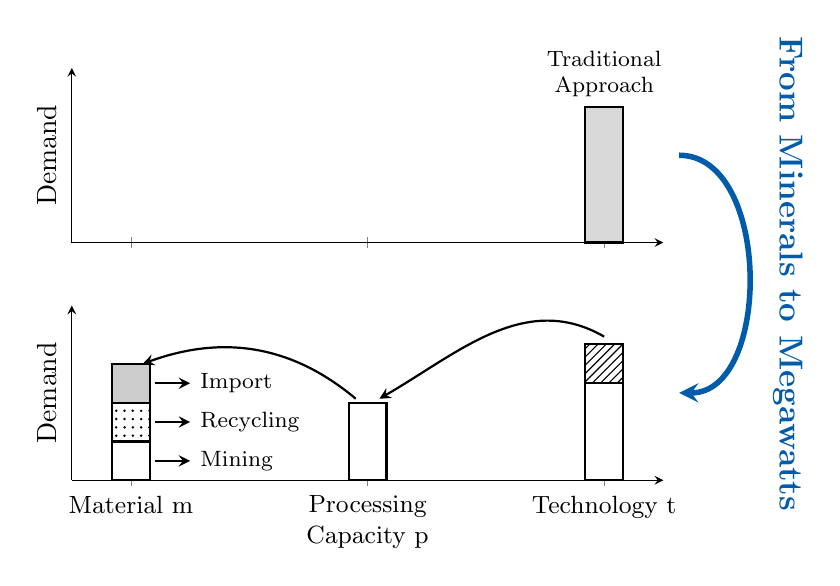
\begin{tikzpicture}
        
                % --- 1. Top Graph ---
                \begin{axis}[
                    name=plot1,
                    width=0.75\textwidth, 
                    height=3.8cm,      % Reduced from 4.5cm to save vertical space
                    axis lines=left,   
                    ylabel={Demand},    
                    ytick=\empty,      
                    xtick={0, 10, 20}, 
                    xticklabels={,,},  
                    ymin=0, ymax=4.5,  
                    xmin=-2.5, xmax=22.5, 
                    clip=false
                ]
                    % Bar at 3rd tick (x=20)
                    \draw[fill=gray!30, draw=black, thick] (axis cs:19.2, 0) rectangle (axis cs:20.8, 3.5);
                    \node[above, align=center, font=\footnotesize] at (axis cs:20, 3.5) {Traditional\\Approach};
                \end{axis}
        
                % --- 2. Bottom Graph ---
                \begin{axis}[
                    name=plot3,
                    at={(plot1.south west)}, 
                    anchor=north west,
                    yshift=-0.8cm,     % Tightened vertical gap from -1.2cm
                    width=0.75\textwidth, 
                    height=3.8cm,      % Reduced from 4.5cm
                    axis lines=left,
                    ylabel={Demand},
                    ytick=\empty,      
                    xtick={0, 10, 20}, 
                    xticklabel style={align=center, font=\small}, 
                    xticklabels={Material $m$, {Processing\\Capacity $p$}, Technology $t$}, 
                    ymin=0, ymax=4.5,
                    xmin=-2.5, xmax=22.5, 
                    clip=false
                ]
                    % --- Bar Tick 1 (Material m at x=0): Stacked, total height 3.0 ---
                    
                    % 1. Mining (bottom, height 1.0)
                    \draw[fill=white, draw=black, thick] (axis cs:-0.8, 0) rectangle (axis cs:0.8, 1.0);
                    \draw[->, thick, >=stealth] (axis cs:1.0, 0.5) -- (axis cs:2.5, 0.5) node[right, font=\footnotesize] {Mining};
                    
                    % 2. Recycling (middle, height 1.0 to 2.0)
                    \draw[pattern=dots, draw=black, thick] (axis cs:-0.8, 1.0) rectangle (axis cs:0.8, 2.0);
                    \draw[->, thick, >=stealth] (axis cs:1.0, 1.5) -- (axis cs:2.5, 1.5) node[right, font=\footnotesize] {Recycling};
                    
                    % 3. Import (top, height 2.0 to 3.0)
                    \draw[fill=gray!40, draw=black, thick] (axis cs:-0.8, 2.0) rectangle (axis cs:0.8, 3.0);
                    \draw[->, thick, >=stealth] (axis cs:1.0, 2.5) -- (axis cs:2.5, 2.5) node[right, font=\footnotesize] {Import};
                    
                    
                    % --- Bar Tick 2 (Processing Capacity p at x=10): height 2.5 ---
                    \draw[fill=white, draw=black, thick] (axis cs:9.2, 0) rectangle (axis cs:10.8, 2.0);
                    
                    % --- Bar Tick 3 (Technology t at x=20): total height 3.5 ---
                    \draw[fill=white, draw=black, thick] (axis cs:19.2, 0) rectangle (axis cs:20.8, 2.5);
                    \draw[pattern=north east lines, draw=black, thick] (axis cs:19.2, 2.5) rectangle (axis cs:20.8, 3.5);
        
                    % --- Arc arrows ---
                    % From Technology back to Processing
                    \draw[->, thick, >=stealth] (axis cs:20, 3.7) to[out=150, in=30] (axis cs:10.5, 2.1);
                    
                    % From Processing back to Material
                    \draw[->, thick, >=stealth] (axis cs:9.5, 2.1) to[out=140, in=20] (axis cs:0.5, 3.0);
                    
                \end{axis}
        
                % --- 3. The "Minerals to Megawatts" Half-Circle Arrow ---
                \draw[->, metublue, line width=2pt, >=stealth] 
                    ([xshift=0.2cm]plot1.east) 
                    to[bend left=90] 
                    node[midway, xshift=0.5cm, font=\bfseries\large, rotate=-90] {From Minerals to Megawatts} 
                    ([xshift=0.2cm]plot3.east);
        
            \end{tikzpicture}
        }
    \end{figure}
\end{frame}

\iffalse
\begin{frame}{Linking processing to final deployement}
    This methodology fundamentally builds upon our previous work\footnote{\tiny Zwickl-Bernhard et al. (2026) \textit{Extending energy system models to assess technology sourcing and resilience}}.
    
    \vspace{0.3cm}
    
    \begin{table}[H]
        \centering
        \renewcommand{\arraystretch}{1.6}
        \scalebox{0.70}{
        \begin{tabular}{l l}
            \toprule
            \textcolor{metublue}{\textbf{Constraint Focus}} & \textcolor{metublue}{\textbf{Mathematical Formulation}} \\
            \midrule
            Linking Supply to Final Deployement & $\hat{\pi}^{\mathrm{new}}_{y,\ell,k} = \hat{\mathcal{Q}}^{\mathrm{supply}}_{y,\ell,k,i=\mathrm{final}}$ \\
            
            Composition of Supply for each Stage \textit{i} & $\hat{\mathcal{Q}}^{\mathrm{supply}}_{y,\ell,k,i} = \hat{q}^{\mathrm{produced}}_{y,\ell,k,i} + \hat{q}^{\mathrm{imported}}_{y,\ell,k,i}$ \\
            
            Linking subsequent Stages until final stage is reached & $\hat{\mathcal{Q}}^{\mathrm{supply}}_{y,\ell,k_{\mathrm{in}},i_{\mathrm{in}}} \geq \sum_{k_{\mathrm{con}}} \sum_{i_{\mathrm{con}}} \hat{q}^{\mathrm{produced}}_{y,\ell,k_{\mathrm{con}},i_{\mathrm{con}}} \times \alpha_{(k_{\mathrm{con}},i_{\mathrm{con}}) \to (k_{\mathrm{in}},i_{\mathrm{in}})}$ \\
            
            Produciton is limited by facility size& $\hat{q}^{\mathrm{produced}}_{y,\ell,k,i} \leq \hat{P}^{\mathrm{proc}}_{y,\ell,k,i}$ \\
            
            Capacity Growth Limit & $\hat{p}^{\mathrm{new}}_{y,\ell,k,i} - \hat{p}^{\mathrm{new}}_{y-1,\ell,k,i} \leq \Delta^{\mathrm{grow}}_{\ell,k,i} + \gamma^{\mathrm{grow}}_{\ell,k,i} \cdot \hat{p}^{\mathrm{new}}_{y-1,\ell,k,i}$ \\
            
            determining energy demand by processing & $E^{\mathrm{factory}}_{y,\ell,k} = \sum_{i} \hat{q}^{\mathrm{produced}}_{y,\ell,k,i} \times e^{\mathrm{need}}_{\ell,k,i}$ \\
            \bottomrule
        \end{tabular}
        }
    \end{table}
    
    \vspace{-0.2cm}
    \begin{center}
        \scriptsize \textit{Indices: year $y$, location $\ell$, technology $k$, processing stage $i$}
    \end{center}
\end{frame}
\fi

\begin{frame}{Linking technology \textit{t} to processing \textit{p}}
    
    \textbf{\textcolor{metublue}{Core Concept:}} \textit{Final capacity installation determines required processing capacity and processed output.}
    \vspace{0.2cm}
    
    \begin{table}[H]
        \centering
        \renewcommand{\arraystretch}{2.0}
        \scalebox{0.62}{
        \begin{tabular}{>{\raggedright\arraybackslash}p{0.45\textwidth} | >{\raggedright\arraybackslash}p{0.75\textwidth}}
            \textcolor{metublue}{\textbf{Constraint Focus}} & \textcolor{metublue}{\textbf{Mathematical Formulation}} \\
            \toprule
            
            Linking supply to final deployment & 
            $\displaystyle \hat{\pi}^{\mathrm{new}}_{y,\ell,k} = \hat{\mathcal{Q}}^{\mathrm{supply}}_{y,\ell,k,i=\mathrm{final}}$ \hfill (1) \\
            
            \rowcolor{metublue!10}
            Composition of supply for each stage $i$ & 
            $\displaystyle \hat{\mathcal{Q}}^{\mathrm{supply}}_{y,\ell,k,i} = \hat{q}^{\mathrm{produced}}_{y,\ell,k,i} + \hat{q}^{\mathrm{imported}}_{y,\ell,k,i}$ \hfill (2) \\
            
            Linking subsequent stages until final stage is reached & 
            $\displaystyle \hat{\mathcal{Q}}^{\mathrm{supply}}_{y,\ell,k,i} \geq \sum_{k',i'} \hat{q}^{\mathrm{produced}}_{y,\ell,k',i'} \times \alpha_{k',i' \to k,i}$ \hfill (3) \\
            
            \rowcolor{metublue!10}
            Production is limited by facility size & 
            $\displaystyle \hat{q}^{\mathrm{produced}}_{y,\ell,k,i} \leq \hat{P}^{\mathrm{proc}}_{y,\ell,k,i}$ \hfill (4) \\
            
            %Capacity growth limit &
            %$\displaystyle \hat{p}^{\mathrm{new}}_{y,\ell,k,i} - \hat{p}^{\mathrm{new}}_{y-1,\ell,k,i} \leq \Delta^{\mathrm{grow}}_{\ell,k,i} + \gamma^{\mathrm{grow}}_{\ell,k,i} \cdot \hat{p}^{\mathrm{new}}_{y-1,\ell,k,i}$ \hfill (5) \\
            
            %\rowcolor{metublue!10}
            Energy consumption of processing facilities & 
            $\displaystyle E^{\mathrm{proc}}_{y,\ell,k} = \sum_{i} \hat{q}^{\mathrm{produced}}_{y,\ell,k,i} \times e^{\mathrm{need}}_{\ell,k,i}$ \hfill (6) \\
            \bottomrule
        \end{tabular}
        }
    \end{table}
    
    \vspace{-0.2cm}
    \begin{center}
        \scriptsize \textit{Indices: year $y$, location $\ell$, technology $k$, processing stage $i$}
    \end{center}
\end{frame}

\begin{frame}{Linking processing \textit{p} to material \textit{m}}
    
    \textbf{\textcolor{metublue}{Core Concept:}} \textit{Processing endogenizes material demand and determines cost-optimal sourcing.}
    \vspace{0.2cm}

    \begin{table}[H]
        \centering
        \renewcommand{\arraystretch}{2.0}
        \scalebox{0.70}{
        \begin{tabular}{>{\raggedright\arraybackslash}p{0.35\textwidth} | >{\raggedright\arraybackslash}p{0.80\textwidth}}
            \textcolor{metublue}{\textbf{Constraint Focus}} & \textcolor{metublue}{\textbf{Mathematical Formulation}} \\
            \toprule
            
            Determine material demand via $\mu$ &
            $\displaystyle D^{\mathrm{mat}}_{y,r} = \sum_{\ell, k, i} \hat{q}^{\mathrm{produced}}_{y,\ell,k,i} \times \mu_{k,i,r}$ \hfill (7) \\
            
            \rowcolor{metublue!10}
            Material sourcing options &
            $\displaystyle D^{\mathrm{mat}}_{y,r} = \hat{m}^{\mathrm{imp}}_{y,r} + \hat{m}^{\mathrm{mine}}_{y,r} + \hat{m}^{\mathrm{rec}}_{y,r}$ \hfill (8) \\
            
            Primary material availability limit &
            $\displaystyle \hat{m}^{\mathrm{mine}}_{y,r} \leq \frac{M^{\mathrm{avail}}_{y,r} \times s^{\mathrm{ET}}_{y,r}}{c^{\mathrm{mine}}_{y,r}}$ \hfill (9) \\
            
            \rowcolor{metublue!10}
            Steady mining growth and decline &
            $\displaystyle 0.70 \times \hat{m}^{\mathrm{mine}}_{y-1,r} \leq \hat{m}^{\mathrm{mine}}_{y,r} \leq 1.30 \times \hat{m}^{\mathrm{mine}}_{y-1,r}$ \hfill (10) \\
            
            Secondary sourcing via $\hat{q}^{\mathrm{rec}}_{y,\ell,k}$ &
            $\displaystyle \hat{m}^{\mathrm{rec}}_{y,r} = \sum_{\ell, k} \hat{q}^{\mathrm{rec}}_{y,\ell,k} \times \frac{\phi_{k,r}}{f^{\mathrm{scrap}}_{\ell,k}} \times \eta^{\mathrm{rec}}_{k,r}$ \hfill (11) \\
            \bottomrule
        \end{tabular}
        }
    \end{table}
    
    \vspace{-0.2cm}
    \begin{center}
        \scriptsize \textit{Indices: year $y$, location $\ell$, technology $k$, processing stage $i$, raw material $r$}
    \end{center}
\end{frame}

\begin{frame}{Retrieving Recycled Materials}
    
    \textbf{\textcolor{metublue}{Core Concept:}} \textit{Decommissioned capacity is re-introduced into the system as scrap, closing the loop, serving as source for recycled materials.}
    \vspace{0.2cm}

    \begin{table}[H]
        \centering
        \renewcommand{\arraystretch}{2.0}
        \scalebox{0.70}{
        \begin{tabular}{>{\raggedright\arraybackslash}p{0.35\textwidth} | >{\raggedright\arraybackslash}p{0.80\textwidth}}
            \textcolor{metublue}{\textbf{Constraint Focus}} & \textcolor{metublue}{\textbf{Mathematical Formulation}} \\
            \toprule
            
            Capacity balance tracking decommissioning &
            $\displaystyle \pi_{y,\ell,k} = \pi_{y-1,\ell,k} + \hat{\pi}^{\mathrm{new}}_{y,\ell,k} - \hat{\pi}^{\mathrm{dec}}_{y,\ell,k}$ \hfill (12) \\
            
            \rowcolor{metublue!10}
            Scrap generation via scrap content $f^{\mathrm{scrap}}_{\ell,k}$ &
            $\displaystyle \hat{q}^{\mathrm{scrap,dec}}_{y,\ell,k} = f^{\mathrm{scrap}}_{\ell,k} \times \hat{\pi}^{\mathrm{dec}}_{y,\ell,k}$ \hfill (13) \\
            
            Total scrap is reduced by recycled mass $\hat{q}^{\mathrm{rec}}_{y,\ell,k}$ &
            $\displaystyle \hat{q}^{\mathrm{scrap,tot}}_{y,\ell,k} = \hat{q}^{\mathrm{scrap,tot}}_{y-1,\ell,k} + \hat{q}^{\mathrm{scrap,dec}}_{y,\ell,k} - \hat{q}^{\mathrm{rec}}_{y,\ell,k}$ \hfill (14) \\
            
            \rowcolor{metublue!10}
            Different options for recycling wind scrap &
            $\displaystyle \hat{q}^{\mathrm{rec}}_{y,\ell,k} = \hat{q}^{\mathrm{rec,mag}}_{y,\ell,k} + \hat{q}^{\mathrm{rec,bulk}}_{y,\ell,k}$ \hfill (15) \\
            \bottomrule
        \end{tabular}
        }
    \end{table}
    
    \vspace{-0.2cm}
    \begin{center}
        \scriptsize \textit{Indices: year $y$, location $\ell$, technology $k$}
    \end{center}
\end{frame}

\begin{frame}{Example: Economies of scale for the recycling sector}
    
    \begin{enumerate}
        \item \textbf{Cumulative Output Tracking:} Track historical experience via past recycled quantities.
        \[ \hat{q}^{\mathrm{cum,rec}}_{y,\ell,k} = \sum_{y'=y_0}^{y} \hat{q}^{\mathrm{rec}}_{y',\ell,k} \]
        
        \item \textbf{Stage Selection via Binary Variable:} A binary variable $\delta_{y,\ell,k,n}$ is activated when the cumulative output crosses a defined threshold ($\hat{Q}^{\mathrm{step}}_{\ell,k,n}$), locking the sector into a specific cost-reduction stage $n$.
        
        \item \textbf{Big-M Linearization:} The auxiliary variable $\hat{z}_{y,\ell,k,n}$ represents the linearized product of the recycling volume and the active stage ($\hat{q}^{\mathrm{rec}}_{y,\ell,k} \cdot \delta_{y,\ell,k,n}$).
        
        \item \textbf{Cost Reduction:} The total cost reduction is given by the active stage discount.
        \[ \Xi^{\mathrm{red}}_{y,\ell,k} = \sum_{n} P^{\mathrm{red}}_{\ell,k,n} \hat{z}_{y,\ell,k,n} \]
    \end{enumerate}
\end{frame}

\begin{frame}{Scenario Constraints: NZIA \& CRMA}
    \begin{itemize}
        \item \textcolor{metublue}{\textbf{Net-Zero Industry Act:}}
    \end{itemize}

    \begin{equation}
    \hat{q}^{\mathrm{flow,dom}}_{y,\ell,k,i} + \hat{q}^{\mathrm{stockout,dom}}_{y,\ell,k,i} \geq 0.40 \times \hat{\mathcal{Q}}^{\mathrm{supply}}_{y,\ell,k,i}
    \label{eq:nzia-constraint}
    \end{equation}

    \vspace{0.5cm}

    \begin{itemize}
        \item \textcolor{metublue}{\textbf{Critical Raw Materials Act:}} %scenario-dependent target ($\chi^{\mathrm{crma}}$).
    \end{itemize}

    \begin{equation}
    \hat{m}^{\mathrm{mine}}_{y,r} + \hat{m}^{\mathrm{rec}}_{y,r} \geq \chi^{\mathrm{crma}} \times D^{\mathrm{mat}}_{y,r}
    \label{eq:crma-constraint}
    \end{equation}
\end{frame}




\section{Results}

% ----- Final Capacities -----
\begin{frame}{Final Installed Capacities: Combined Relative Change}
    \begin{figure}
        \centering
        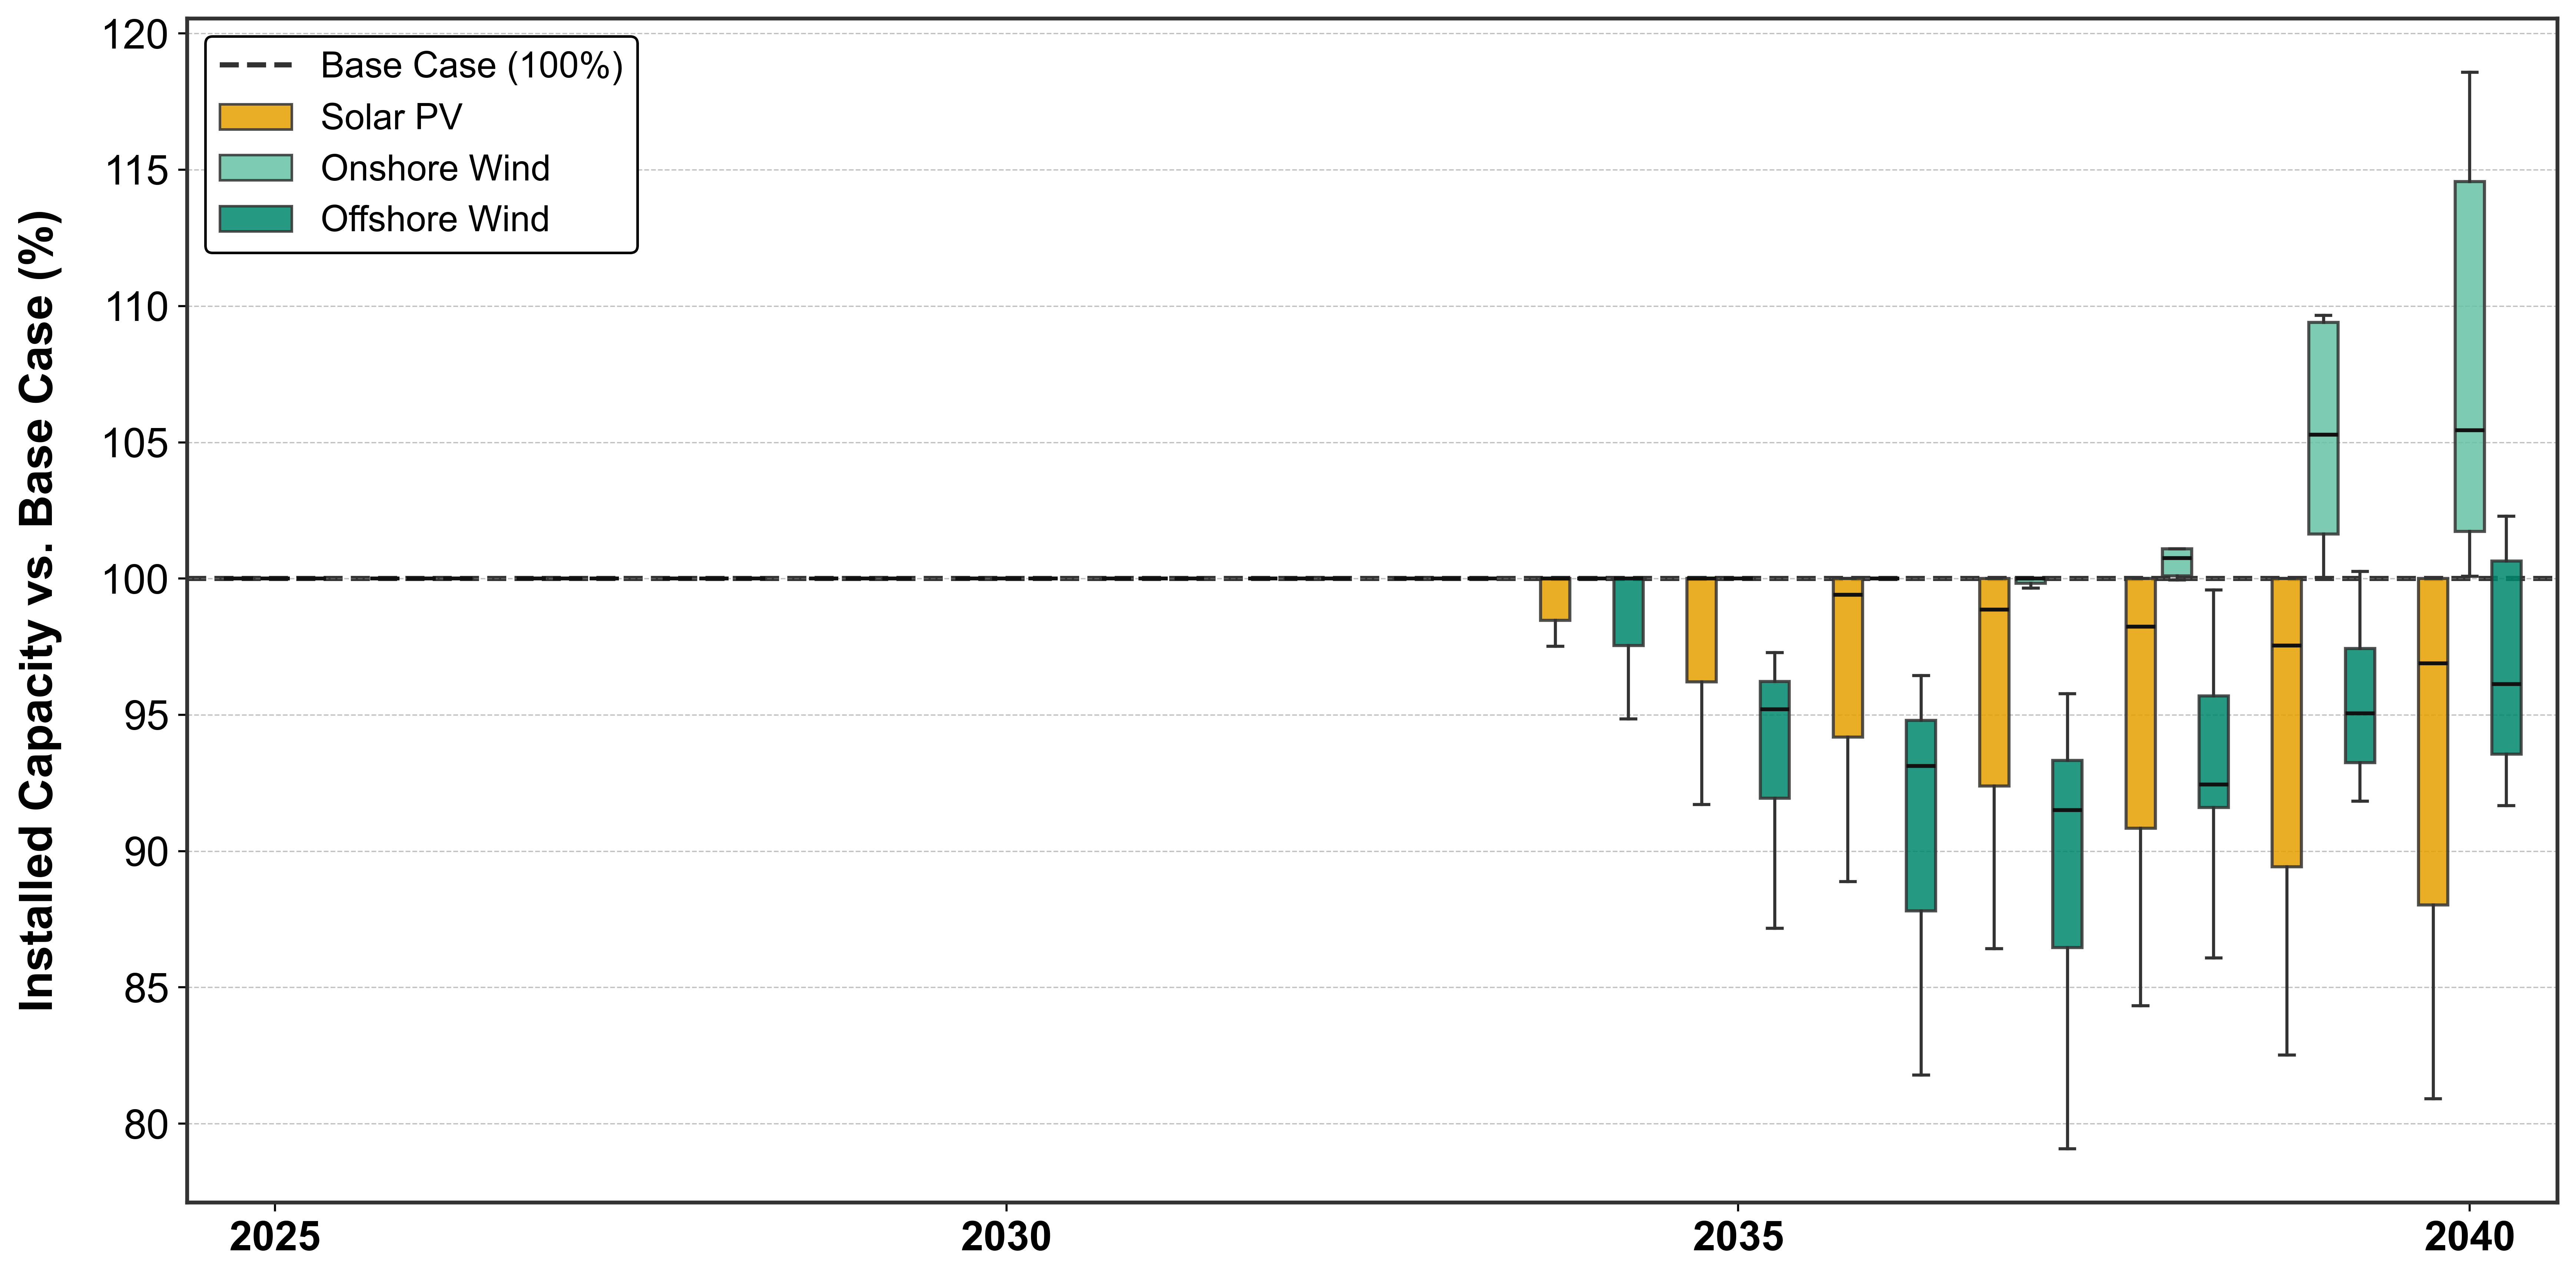
\includegraphics[width=1\linewidth,height=0.85\textheight,keepaspectratio]{../plot_iew/final_capacities/Capacities_Combined_Relative_Boxplot.png}
    \end{figure}
\end{frame}

% ----- Processing Capacities -----
\begin{frame}{Processing Capacities: Solar PV}
    \begin{figure}
        \centering
        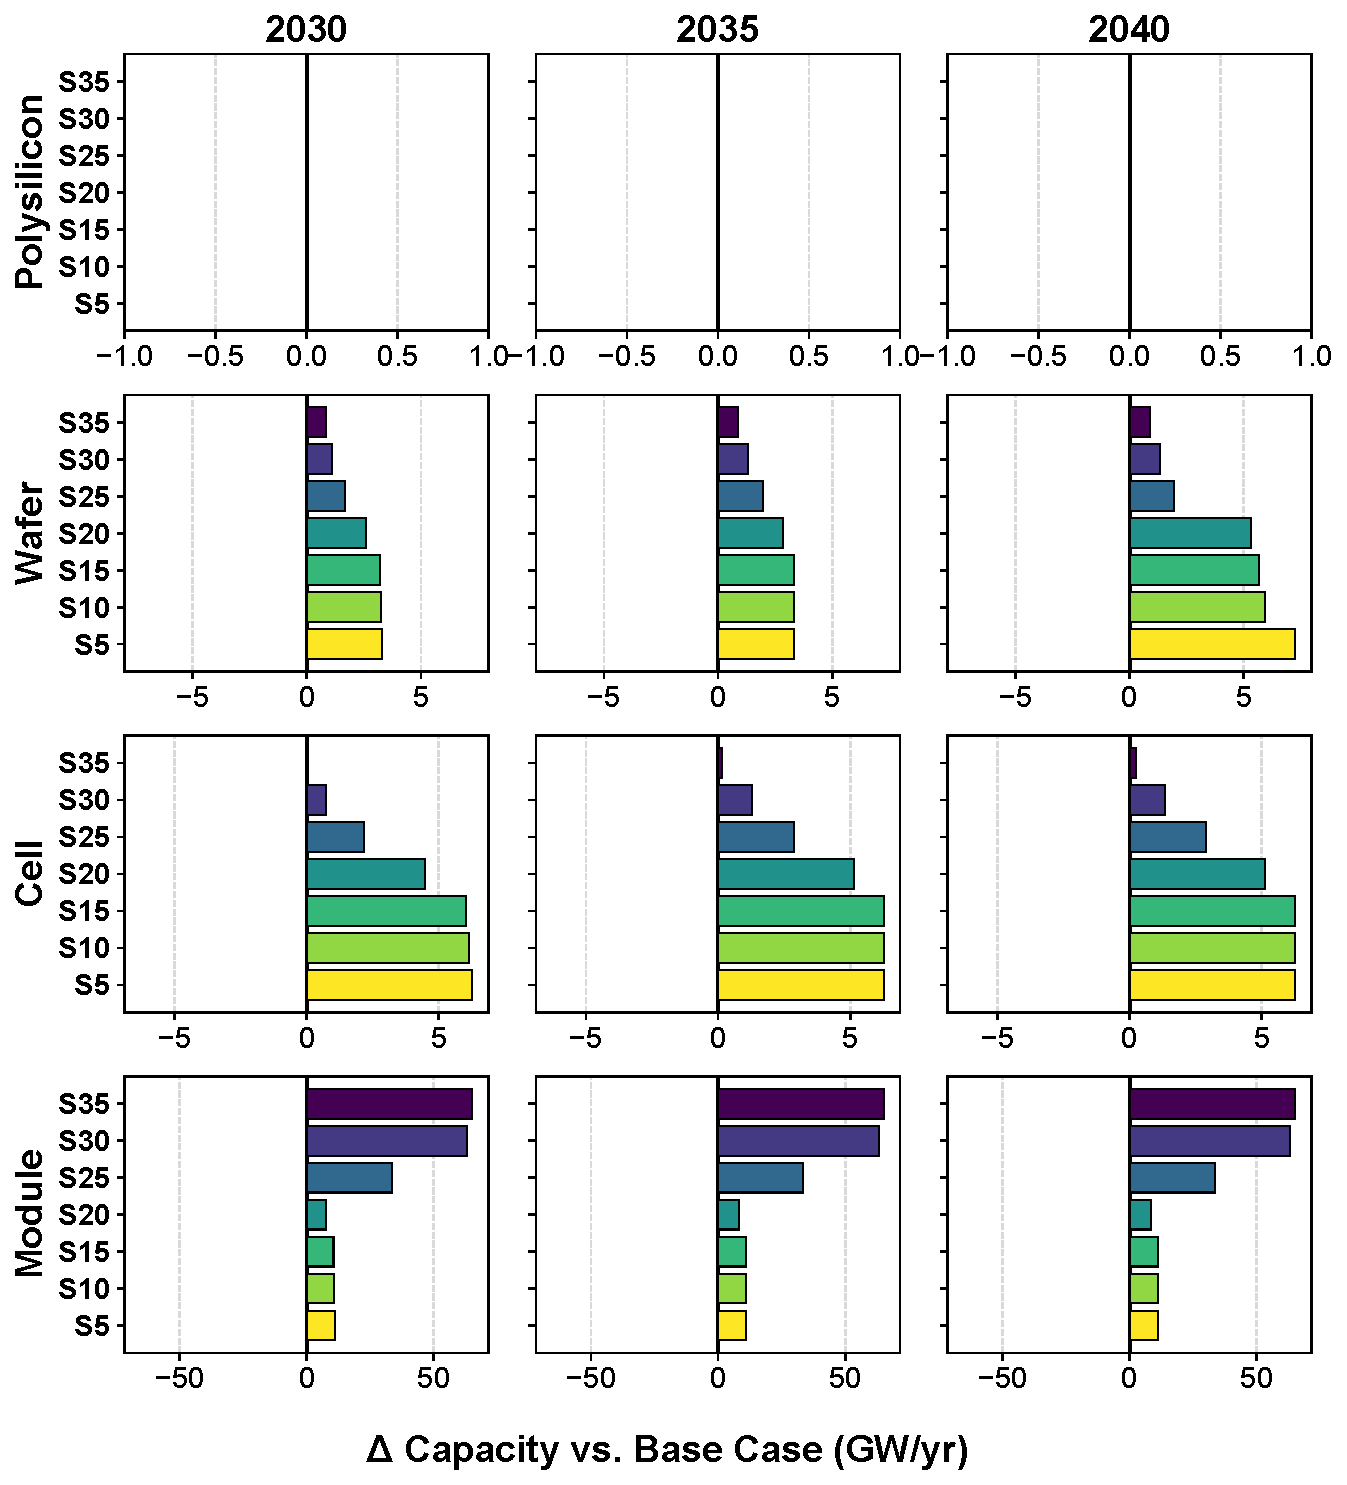
\includegraphics[width=1\linewidth,height=0.85\textheight,keepaspectratio]{../plot_iew/processing_capacities/Diverging_Delta_solarPV.pdf}
    \end{figure}
\end{frame}

\begin{frame}{Processing Capacities: Wind Onshore}
    \begin{figure}
        \centering
        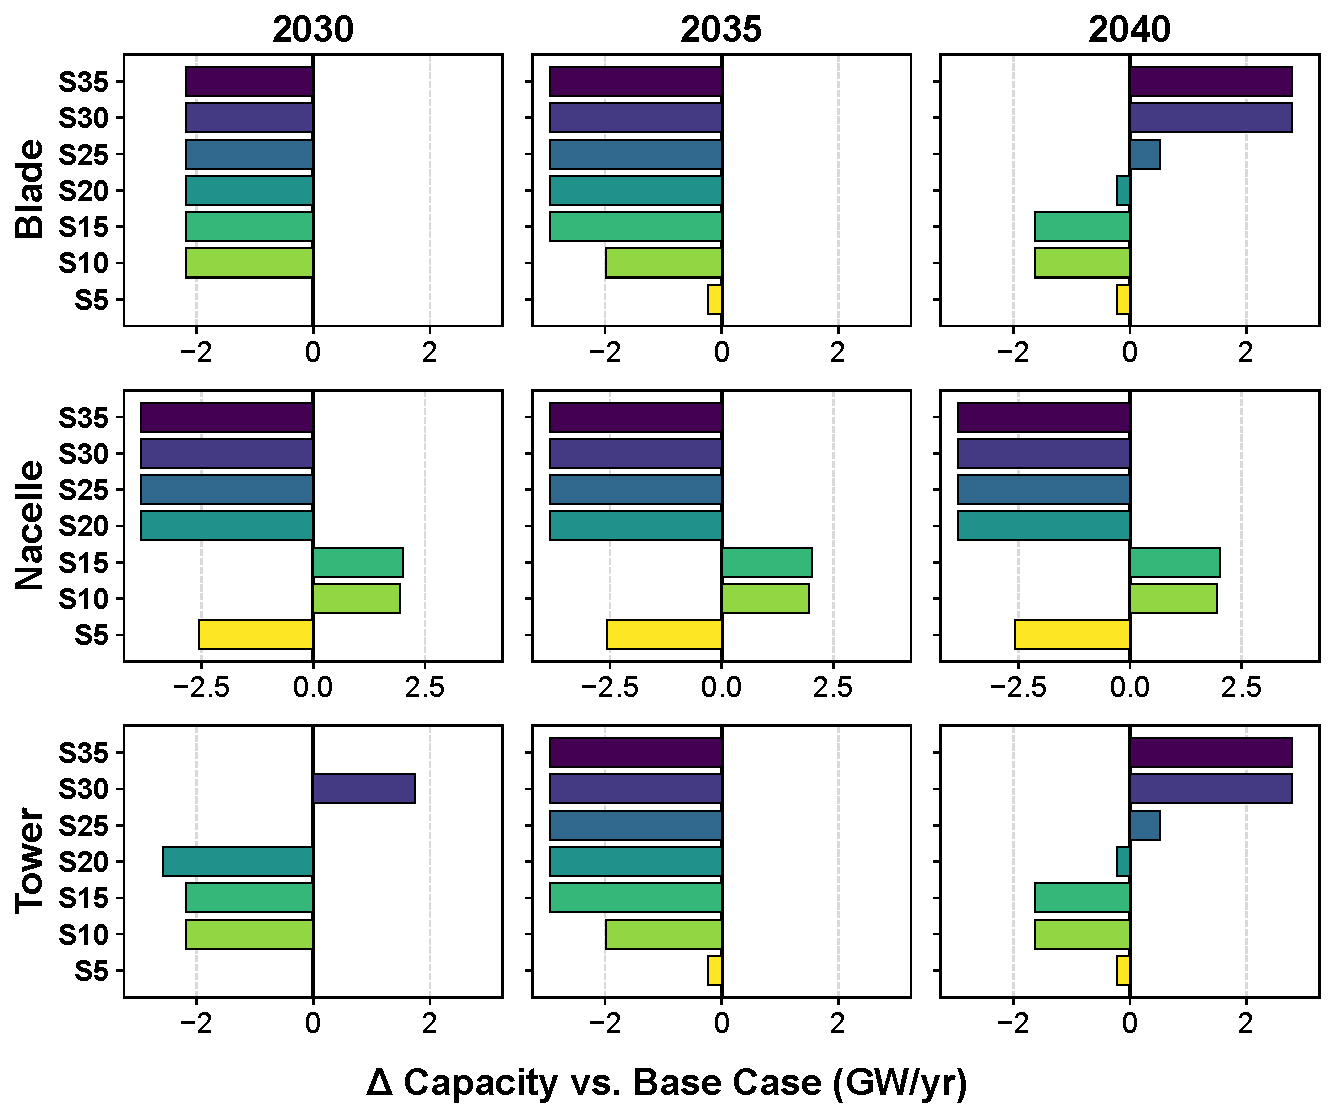
\includegraphics[width=1\linewidth,height=0.85\textheight,keepaspectratio]{../plot_iew/processing_capacities/Diverging_Delta_windon.pdf}
    \end{figure}
\end{frame}

\begin{frame}{Processing Capacities: Wind Offshore}
    \begin{figure}
        \centering
        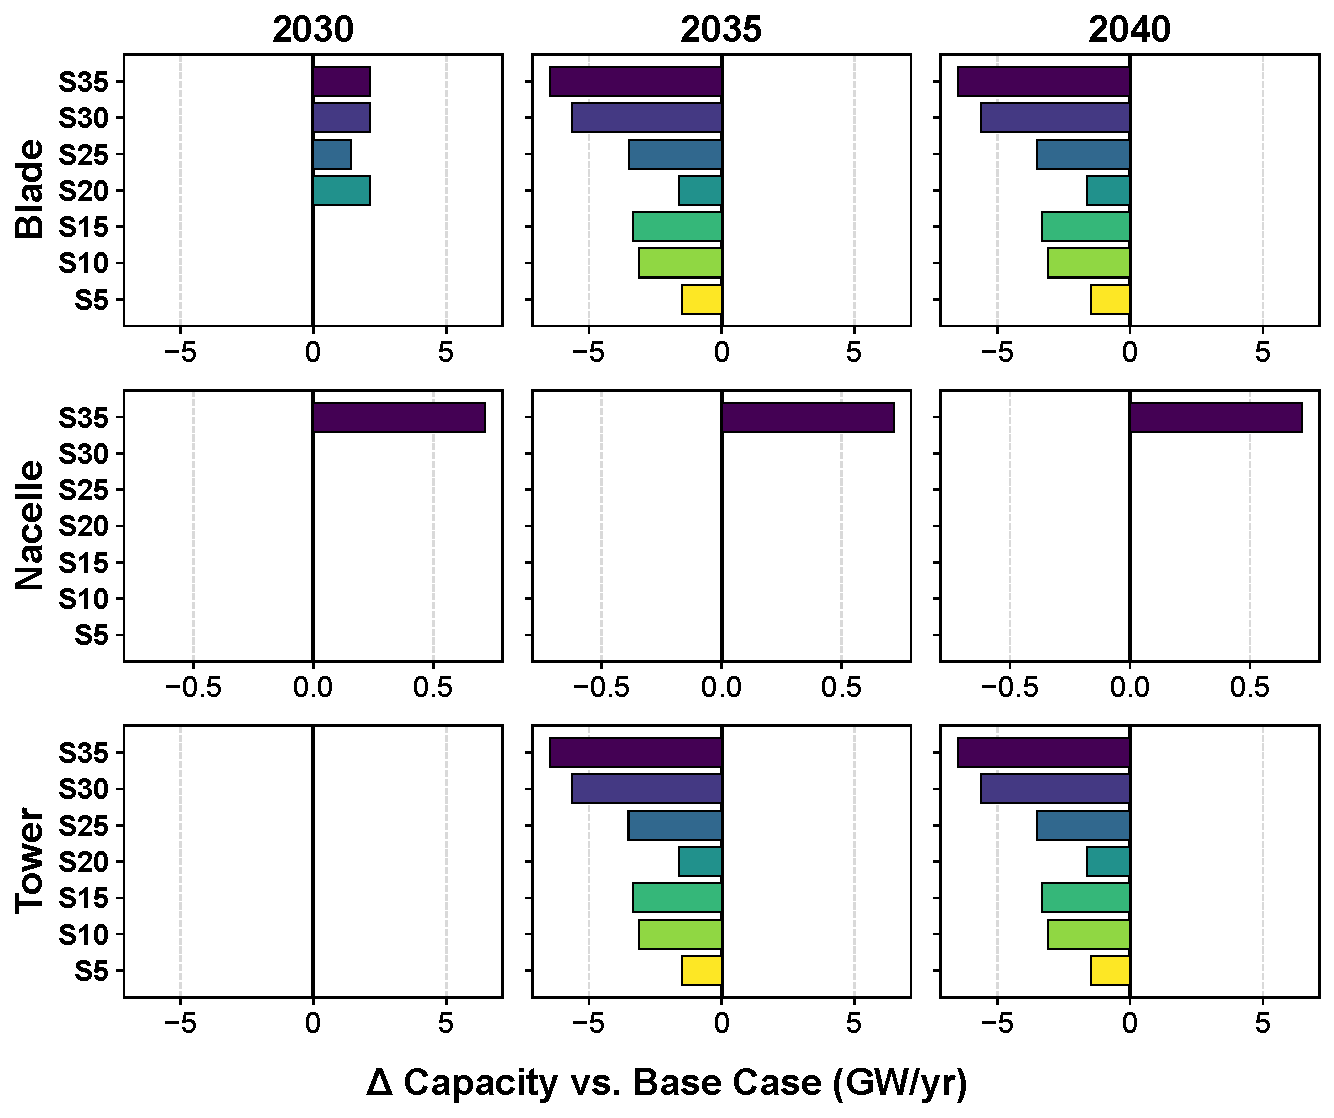
\includegraphics[width=1\linewidth,height=0.85\textheight,keepaspectratio]{../plot_iew/processing_capacities/Diverging_Delta_windoff.pdf}
    \end{figure}
\end{frame}

% ----- Materials Sourcing -----
%\begin{frame}{Critical Raw Materials Sourcing}
%    \begin{figure}
%        \centering
%        \includegraphics[height=0.85\textheight]{../plot_iew/minerals_sourcing/Domestic_Sourcing_Radar_Grid.png}
%    \end{figure}
%\end{frame}

\begin{frame}{CRM Sourcing: Selected Examples}
    \begin{figure}
        \centering
        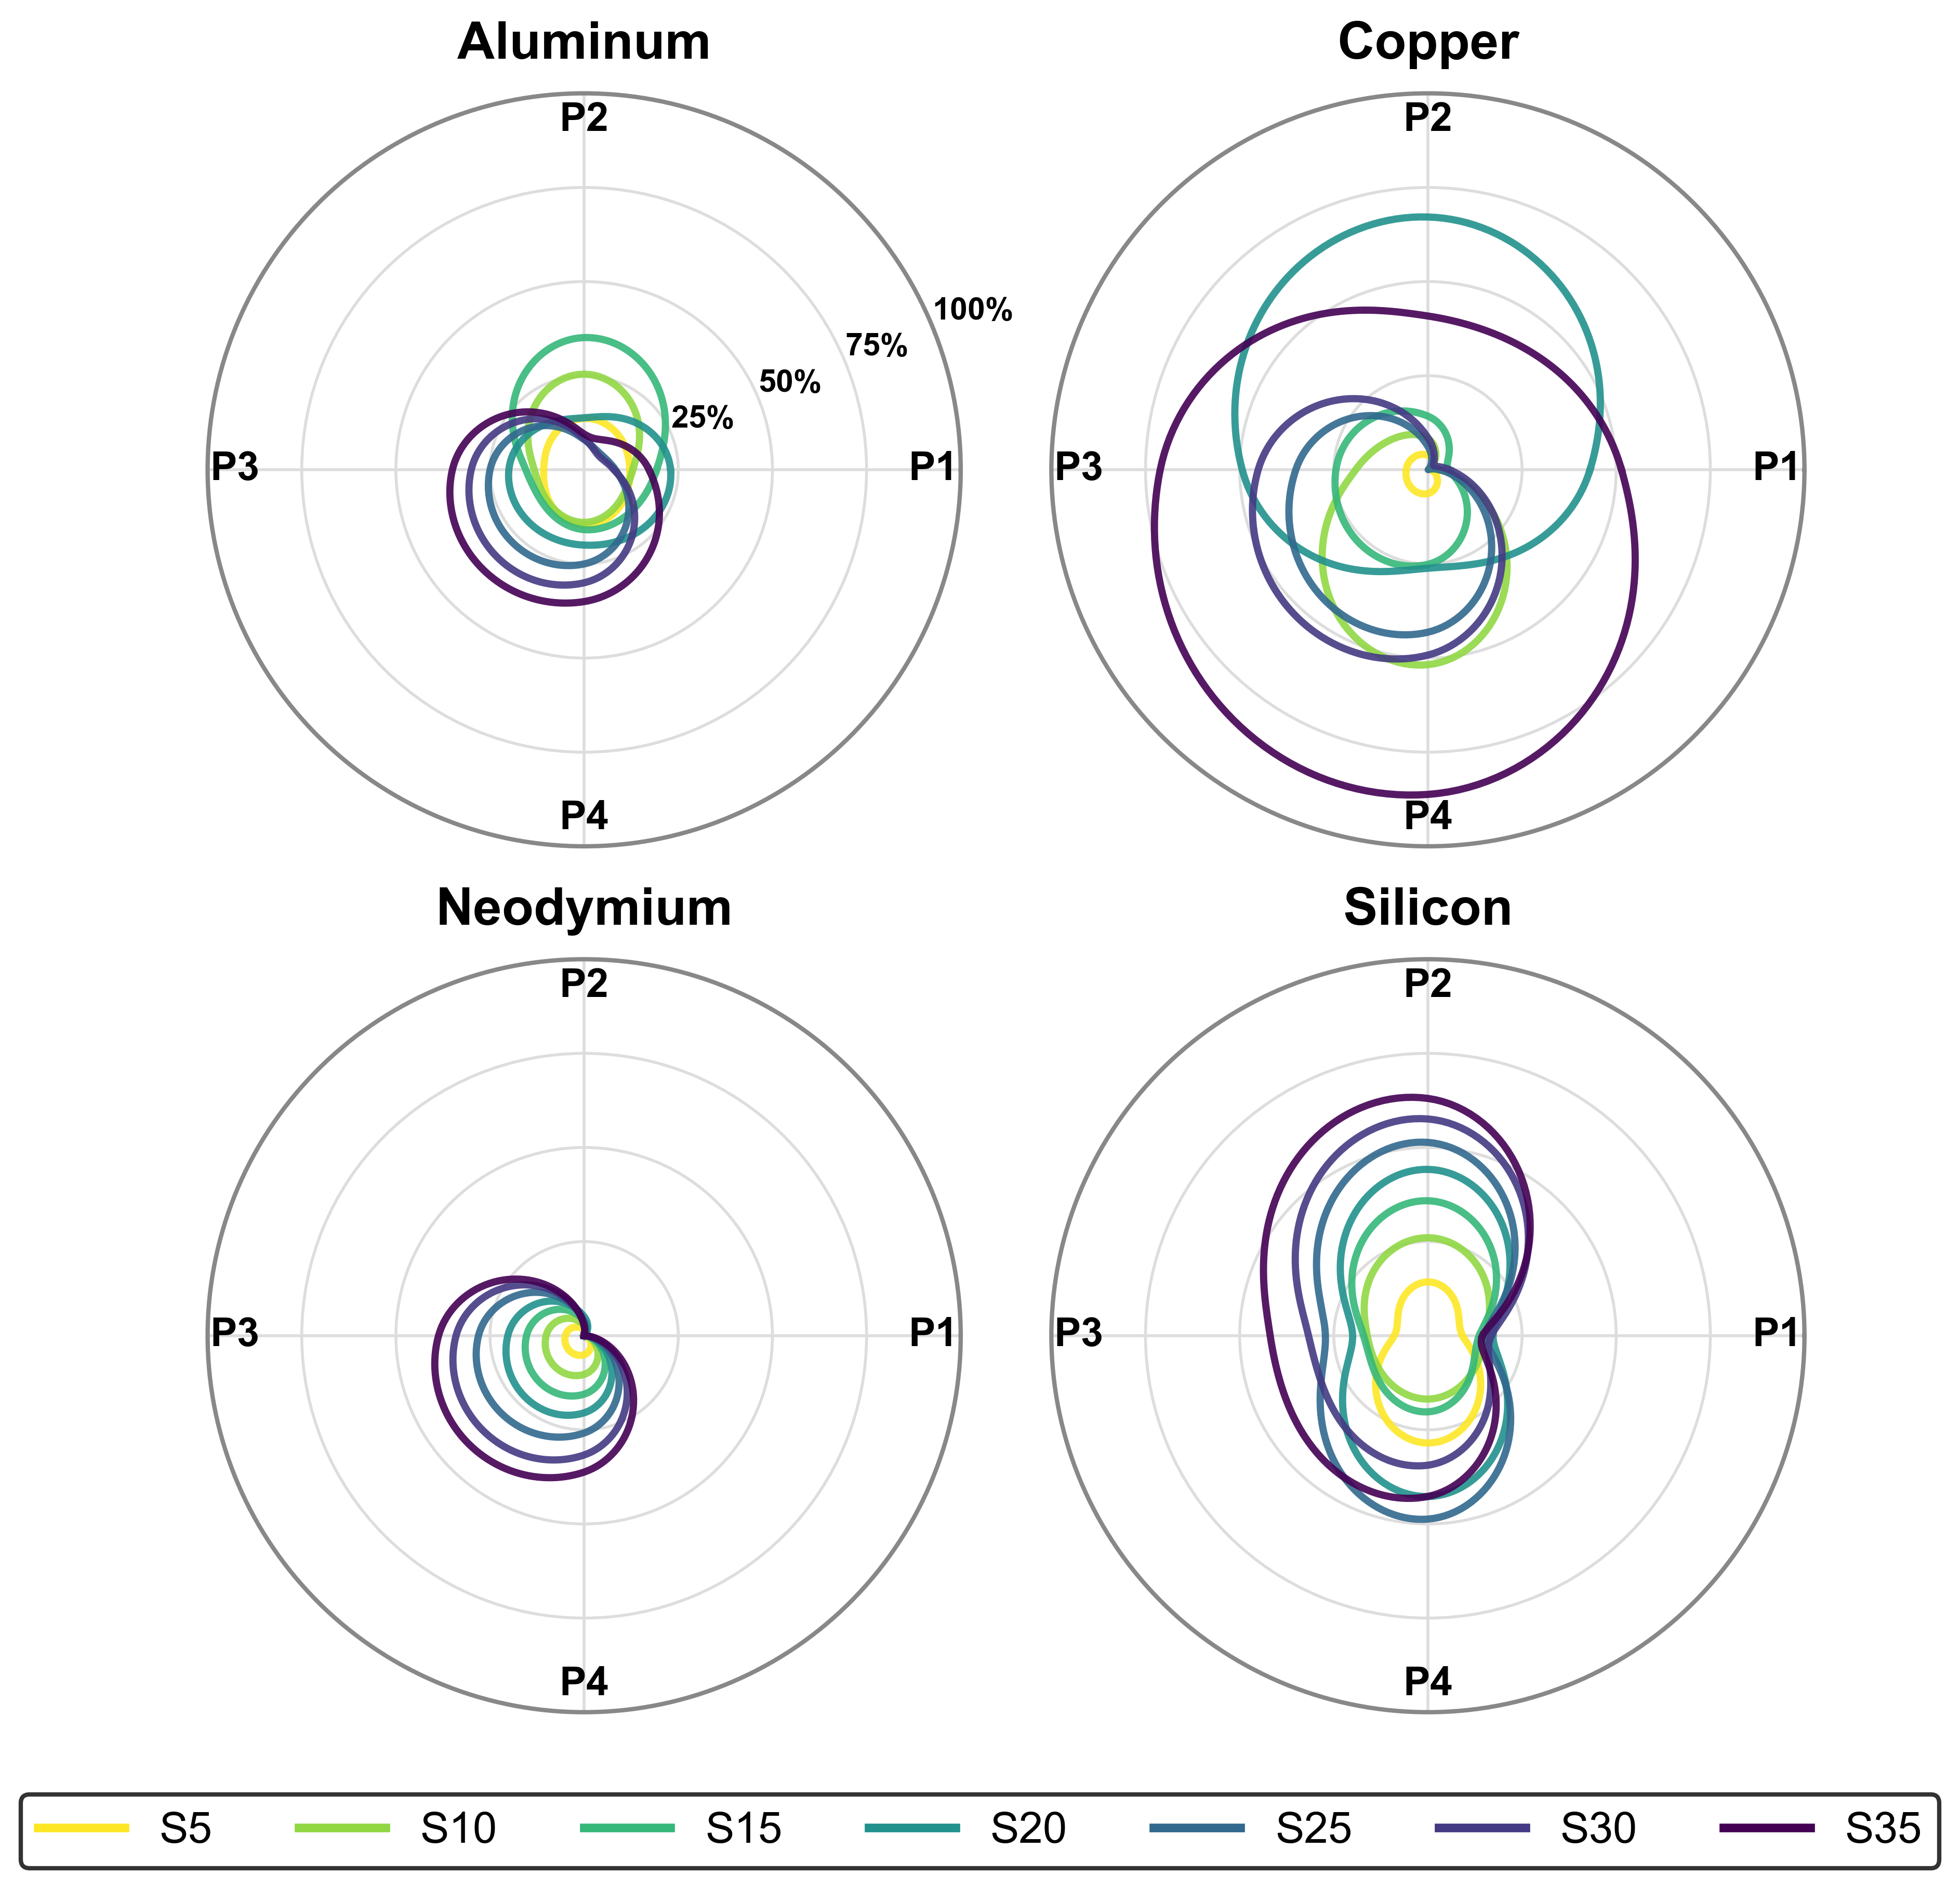
\includegraphics[height=0.85\textheight,keepaspectratio]{../plot_iew/minerals_sourcing/individual_radars/Selected_Examples_Grid.png}
    \end{figure}
\end{frame}

\section{Conclusion}
\begin{frame}{Conclusion}

\begin{itemize}
        \item \textcolor{metublue}{\textbf{Proof of Concept:}} The energy-material nexus is successfully endogenized, even under severe data scarcity.
        \item \textcolor{metublue}{\textbf{Policy Coordination:}} Industrial and material targets must be aligned; weak mandates fail to incentivize domestic processing (e.g., Wind).
        \item \textcolor{metublue}{\textbf{Capacity Patterns:}} Cross-technology materials exhibit complex interactions requiring deeper study. Solar PV is the preferred choice in low CRMA scenarios, whereas for wind, the opposite is true.
        \item \textcolor{metublue}{\textbf{Unexpected Pathways:}} The model determines CCUS technology as cost-optimal option for electricity decarbonization.
    \end{itemize}
\end{frame}

\begin{frame}{Future Work \& Next Steps}
    \begin{table}
        \centering
        \begin{tabular}{p{0.46\linewidth} | p{0.46\linewidth}}
            \textcolor{metublue}{\textbf{Pathway A: Data Scarcity Resolved}} & \textcolor{metublue}{\textbf{Pathway B: Data Scarcity Persists}} \\
            \midrule
            \vspace{-0.4cm}
            \begin{itemize}
                \item Obtain exact CRM price trajectories and recycling costs.
                \item Shift focus to granular geographic modeling (higher solve times).
                \item Apply methodology to other sectors (e.g., EV batteries).
            \end{itemize}
            & 
            \vspace{-0.4cm}
            \begin{itemize}
                \item Use massive scenario runs to map parameter uncertainty.
                \item Keep model strictly linear to guarantee fast solve times.
                \item Explore soft-linking to prevent non-linear LP-bottlenecks.
            \end{itemize} \\
        \end{tabular}
    \end{table}
\end{frame}

\begin{frame}[plain] 
    \centering
    \vspace*{1.5cm}

    % Define it here using RGB if not defined globally
    \definecolor{metublue}{RGB}{0, 92, 171}

    {\Huge \textcolor{metublue}{\textbf{Thank You}}} \\[0.5cm]
    {\Large for your attention.}

    \vspace{1.5cm}

    {\Large Happy to answer your questions!}

    \vspace{0.8cm}

    {\large Find out more about us at: \href{https://es3m.eu}{\textbf{\textcolor{metublue}{es3m.eu}}}}

    \vspace{0.5cm}

    \vfill

    {\footnotesize \textit{\textcolor{gray}{oitzinger@eeg.tuwien.ac.at}}}
    \vspace*{0.5cm}
\end{frame}

\appendix

%%\section*{Reference}
%------------------------------------------------% 
%\begin{frame}[t,allowframebreaks]{References}
%    \begin{small}
%        \bibliographystyle{unsrtnat}
%        \bibliography{bibliography}
%    \end{small}
%\end{frame}

\iffalse
% --- BACKUP OF COMPACT TABLE METHODS SLIDES (First Iteration) ---
\begin{frame}{Linking processing to final deployement}
    This methodology fundamentally builds upon our previous work\footnote{\tiny Zwickl-Bernhard \& Oitzinger (2025) \textit{Securing EU Clean Technology Supply Chains}}.
    
    \vspace{0.3cm}
    
    \begin{table}[H]
        \centering
        \renewcommand{\arraystretch}{1.6}
        \scalebox{0.70}{
        \begin{tabular}{l l}
            \toprule
            \textcolor{metublue}{\textbf{Constraint Focus}} & \textcolor{metublue}{\textbf{Mathematical Formulation}} \\
            \midrule
            Final Capacity Link & $\hat{\pi}^{\mathrm{new}}_{y,\ell,k} = \hat{\mathcal{Q}}^{\mathrm{supply}}_{y,\ell,k,i=\mathrm{final}}$ \\
            
            Composition of Supply & $\hat{\mathcal{Q}}^{\mathrm{supply}}_{y,\ell,k,i} = \left(\hat{q}^{\mathrm{flow,dom}}_{y,\ell,k,i} + \hat{q}^{\mathrm{stockout,dom}}_{y,\ell,k,i}\right) + \left(\hat{q}^{\mathrm{flow,imp}}_{y,\ell,k,i} + \hat{q}^{\mathrm{stockout,imp}}_{y,\ell,k,i}\right)$ \\
            
            Production Limits & $\hat{q}^{\mathrm{produced}}_{y,\ell,k,i} \leq \hat{P}^{\mathrm{proc}}_{y,\ell,k,i}$ \\
            
            Stage Linkage (BOM) & $\hat{\mathcal{Q}}^{\mathrm{supply}}_{y,\ell,k,i} \geq \sum_{k',i'} \hat{q}^{\mathrm{produced}}_{y,\ell,k',i'} \times \mathrm{BOM}_{k,i \to k',i'}$ \\
            
            Capacity Growth Limit & $\hat{p}^{\mathrm{new}}_{y,\ell,k,i} - \hat{p}^{\mathrm{new}}_{y-1,\ell,k,i} \leq \Delta^{\mathrm{grow}}_{\ell,k,i} + \gamma^{\mathrm{grow}}_{\ell,k,i} \cdot \hat{p}^{\mathrm{new}}_{y-1,\ell,k,i}$ \\
            \bottomrule
        \end{tabular}
        }
    \end{table}
\end{frame}

\begin{frame}{Linking Materials to Processing}
    This module bridges the gap between technology deployment and raw material availability.
    
    \vspace{0.3cm}
    
    \begin{table}[H]
        \centering
        \renewcommand{\arraystretch}{1.6}
        \scalebox{0.70}{
        \begin{tabular}{l l}
            \toprule
            \textcolor{metublue}{\textbf{Constraint Focus}} & \textcolor{metublue}{\textbf{Mathematical Formulation}} \\
            \midrule
            Material Demand & $\hat{q}^{\mathrm{demand,tot}}_{y,\ell,k,r} = \sum_i \hat{q}^{\mathrm{produced}}_{y,\ell,k,i} \times \mu_{k,i,r}$ \\
            
            Material Composition & $D^{\mathrm{mat}}_{y,r} = \hat{m}^{\mathrm{imp}}_{y,r} + \hat{m}^{\mathrm{mine}}_{y,r} + \hat{m}^{\mathrm{rec}}_{y,r}$ \\
            
            Primary Limit & $\hat{m}^{\mathrm{mine}}_{y,r} \leq \frac{M^{\mathrm{avail}}_{y,r} \times s^{\mathrm{ET}}_{y,r}}{c^{\mathrm{mine}}_{y,r}}$ \\
            
            Secondary Sourcing & $\hat{m}^{\mathrm{rec}}_{y,r} = \sum_{\ell, k} \hat{q}^{\mathrm{rec}}_{y,\ell,k} \times \frac{\phi_{k,r}}{f^{\mathrm{scrap}}_{\ell,k}} \times \eta^{\mathrm{rec}}_{k,r}$ \\
            \bottomrule
        \end{tabular}
        }
    \end{table}
\end{frame}

\begin{frame}{Retrieving Recycled Materials}
    \begin{table}[H]
        \centering
        \renewcommand{\arraystretch}{1.6}
        \scalebox{0.70}{
        \begin{tabular}{l l}
            \toprule
            \textcolor{metublue}{\textbf{Constraint Focus}} & \textcolor{metublue}{\textbf{Mathematical Formulation}} \\
            \midrule
            Scrap Generation & $\hat{q}^{\mathrm{scrap,dec}}_{y,\ell,k} = f^{\mathrm{scrap}}_{\ell,k} \times \hat{\mathcal{K}}^{\mathrm{dec}}_{y,\ell,k}$ \\
            
            Scrap Accumulation & $\hat{q}^{\mathrm{scrap,tot}}_{y,\ell,k} = \hat{q}^{\mathrm{scrap,tot}}_{y-1,\ell,k} + \hat{q}^{\mathrm{scrap,dec}}_{y,\ell,k} - \hat{q}^{\mathrm{rec}}_{y,\ell,k}$ \\
            
            Endogenous Recycling & $\hat{q}^{\mathrm{rec}}_{y,\ell,k} = \hat{q}^{\mathrm{rec,mag}}_{y,\ell,k} + \hat{q}^{\mathrm{rec,bulk}}_{y,\ell,k} \quad \forall k \in \{\text{wind}\}$ \\
            \bottomrule
        \end{tabular}
        }
    \end{table}
\end{frame}

\begin{frame}{Example: Economies of Scale}
    Economies of scale are driven by cumulative output over time, dynamically reducing costs as experience grows. For recycling, this builds upon cumulative secondary production:
    
    \vspace{0.3cm}
    \begin{equation}
    \hat{q}^{\mathrm{cum,rec}}_{y,k} = \sum_{y'=y_0}^{y} \hat{q}^{\mathrm{rec}}_{y',\ell,k}
    \label{eq:cum-scrap}
    \end{equation}
    \vspace{0.3cm}
    
    \begin{itemize}
        \item \textcolor{metublue}{\textbf{Cost Reduction:}} Learning rates are applied to $\hat{q}^{\mathrm{cum,rec}}_{y,k}$ to linearly discount the CAPEX and OPEX associated with recycling capacity.
    \end{itemize}
\end{frame}
\fi

\end{document}
